\section{Kriptografi Berbasis Kurva Eliptik}
Inti dari keamanan ECC adalah \textbf{Elliptic Curve Discrete Logarithm Problem (ECDLP)}.

\subsection{ECDLP}
Diberikan titik basis $P$ dan titik $Q$ pada kurva eliptik, sangat sulit untuk menemukan integer $k$ sedemikian sehingga:
\[ Q = kP = \underbrace{P + P + \dots + P}_{k \text{ kali}} \]
Jika $k$ adalah bilangan yang sangat besar, mencari $k$ dari $P$ dan $Q$ secara komputasi tidak praktis.

\subsection{Mekanisme Kunci}
\begin{itemize}
    \item \textbf{Kunci Privat}: Integer acak $k \in [1, p-1]$.
    \item \textbf{Kunci Publik}: Titik $Q = kP$ pada kurva eliptik.
\end{itemize}

\subsection{Protokol Utama}
\begin{enumerate}
    \item \textbf{ECDH (Elliptic Curve Diffie-Hellman)}: Pertukaran kunci rahasia bersama menggunakan operasi perkalian titik.
    \item \textbf{ECEG (Elliptic Curve ElGamal)}: Enkripsi pesan dengan mengkodekan pesan menjadi titik $P_M$ dan menghasilkan cipherteks berupa pasangan titik $[(kB), (P_M + kP_B)]$.
\end{enumerate}

\subsection{Perbandingan dengan RSA}
Keunggulan utama ECC adalah ukuran kunci yang jauh lebih pendek untuk tingkat keamanan yang setara, seperti ditunjukkan pada Tabel~\ref{tab:ecc-vs-rsa}.

\begin{table}[htbp]
    \centering
    \caption{Ukuran kunci ECC dan RSA untuk tingkat keamanan yang setara}
    \label{tab:ecc-vs-rsa}
    \begin{tabular}{|c|c|c|}
    \hline
    \textbf{Keamanan (bit)} & \textbf{Kunci ECC (bit)} & \textbf{Kunci RSA (bit)} \\
    \hline
    80 & 160 & 1024 \\
    \hline
    112 & 224 & 2048 \\
    \hline
    128 & 256 & 3072 \\
    \hline
    192 & 384 & 7680 \\
    \hline
    256 & 512 & 15360 \\
    \hline
    \end{tabular}
\end{table}


\begin{figure}[htbp]
    \centering
    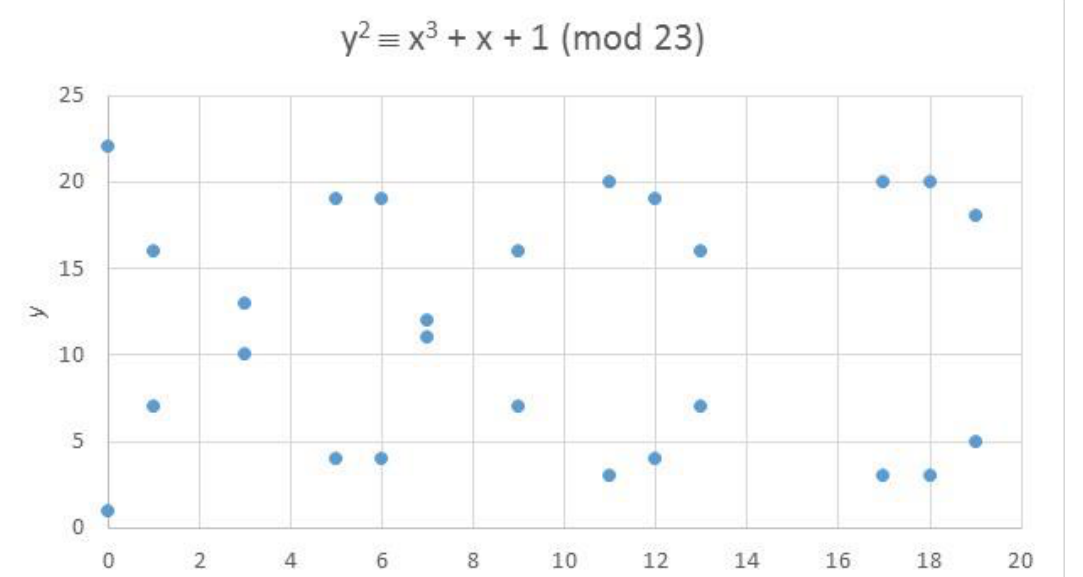
\includegraphics[width=0.6\linewidth, height=0.65\textheight, keepaspectratio]{figures/titik-kurva-mod-23.png}
    \caption{Sebaran titik kurva eliptik $y^2 \equiv x^3 + x + 1 \pmod{23}$; himpunan titik berhingga inilah yang membentuk grup tempat persoalan logaritma diskrit kurva eliptik bekerja}
    \label{fig:titik-kurva-mod-23}
    \sumber{Munir, \textit{IF4020 Kriptografi}, ITB.}
\end{figure}
